\section{Experiments That Validated the Design}
\label{sec:experiments}

The cascade described in Section~\ref{sec:cascade} was not designed in one shot. It is the product of two rounds of experimentation: a \emph{first round} of 13 baseline ablations that locked the cascade structure (we called this lock-in ``v2f''), and a \emph{second round} of 8 targeted late-stage refinements (the G-series) that took us from v2f to the final headline.

We describe both rounds because the negative results in each are informative. Three patterns emerged across the second round that we believe are interesting findings in their own right (Section~\ref{sec:cross-cutting}).

\subsection{Round 1 --- the 13 baseline ablations}

\paragraph{Method.} Thirteen independent ablations were run against the v2f cascade. Each ablation tested one design dimension and was kept or rejected based on the measured delta. Table~\ref{tab:baseline-ablations} summarizes.

\begin{table}[h]
\centering
\caption{The 13 baseline ablations. \textsc{Keep} = the variant improved the cascade and was integrated. \textsc{Reject} = the variant hurt; we kept the simpler design.}
\label{tab:baseline-ablations}
\small
\setlength{\tabcolsep}{4pt}
\renewcommand{\arraystretch}{1.15}
\begin{tabularx}{\linewidth}{@{}r >{\raggedright\arraybackslash}X >{\raggedright\arraybackslash}X@{}}
\toprule
\# & Question & Outcome \\
\midrule
1 & Which retrievers to include in L2 RRF? Drop-one over the six. & \textsc{Drop} Hybrid-RRF-LLM ($+2.1$ pts Hit@5). Keep the other four. \\
2 & Score-weighted RRF (weight by standalone Hit@5)? & All variants hurt by 4--6 pts Hit@5; \textsc{keep} uniform weights. \\
3 & Per-family oracle (assume gold family known, pick best retriever per family)? & Oracle Hit@5 $= 0.888$, \emph{worse} than uniform RRF $0.912$; \textsc{reject}. \\
4 & Confidence-aware RRF (weight by per-window triage)? & Hurts by 5--7 pts Hit@1; \textsc{reject}. \\
5 & Learned per-candidate ranker (LogReg on rank features)? & Hit@5 $= 0.825$, far below cascade $0.912$; \textsc{reject}. \\
6 & Overlap-rerank window sweep (top-3 vs top-5 vs top-10)? & top-3 + 3-voter pool optimal at Hit@1 $= 0.722$; \textsc{keep top-3}. \\
7 & Let DiagnosisAgent override L2 top-1? & Net $-5$ Hit@1 wins on 200 windows; \textsc{disable} agent rerank. \\
8 & L1 stacker: GBM vs LogReg? & LogReg PR-AUC $0.9998 / 0.853$ vs GBM $0.985 / 0.739$; \textsc{keep} LogReg. \\
9 & L1 derived features (max-conf, variance, consensus)? & Inclusive PR-AUC drops $0.853 \to 0.849$; \textsc{reject}. \\
10 & L1 without HGB? & Strict PR-AUC collapses $0.9998 \to 0.303$; HGB is essential. \\
11 & L1 noise threshold sweep $\{0.1, 0.2, 0.3, 0.5\}$? & Recall stays $1.000$, F1 peaks at $\tau = 0.5$; \textsc{use} 0.5. \\
12 & Free novelty signal vs agent's \texttt{is\_novel}? & At $\tau = 0.5$: 96\% precision (matches agent); OR-combine widens recall; \textsc{use combined OR}. \\
13 & Multi-seed stability of stacker (seeds 1, 7, 42, 100, 1000)? & Strict PR-AUC std $= 0.0000$; inclusive std $= 0.0025$; \textsc{not} a fortunate seed. \\
\bottomrule
\end{tabularx}
\end{table}

\paragraph{The theoretical ceiling.} We computed the upper bound of any fusion of the four chosen L2 retrievers: the union of the four top-5 sets contains the gold ticket on 97.6\% of windows. The v2f cascade at Hit@5 $= 0.912$ is at $93.5\%$ of that ceiling. Closing the remaining 6.4-point gap requires a \emph{structurally new retriever} (a different inductive bias), not further fusion tuning. This conclusion motivated the G-series.

\subsection{Round 2 --- the G-series of eight targeted refinements}

The G-series ran in June 2026 with a single explicit goal: close part of the 6.4-point Hit@5 gap, or, failing that, find improvements on the other axes (novelty recall, robustness, OOD generalization). Each phase was committed independently and observed in writing.

\begin{table}[h]
\centering
\caption{G-series outcomes. KEEP-headline $=$ integrated into the final cascade. KEEP-analysis $=$ published as a robustness/generalization result but does not modify the cascade. SKIP $=$ the variant hurt or did not help.}
\label{tab:g-summary}
\small
\setlength{\tabcolsep}{4pt}
\renewcommand{\arraystretch}{1.15}
\begin{tabularx}{\linewidth}{@{}l >{\raggedright\arraybackslash}X >{\raggedright\arraybackslash}X@{}}
\toprule
Phase & Intervention & Verdict \\
\midrule
G1 & BiEncoder fine-tune with BM25 hard-negs + random negs & \textbf{KEEP} (Hit@1 $+2.1\%$ rel) \\
G2 & Fine-tuned cross-encoder as 5th retriever / reranker & SKIP (Hit@1 $-5.4$ pts) \\
G3 & Symmetric LLM extraction (windows too, not just tickets) & SKIP (standalone Hit@1 $+404\%$ rel; cascade integration breaks) \\
G4 & DiagnosisAgent Phase 3: complete coverage on remaining 658 windows & \textbf{KEEP} (novel recall $+119\%$ rel) \\
G5 & LLM judge reranker (Qwen picks best of top-5) & SKIP (third reranker negative; uninformative confidence) \\
G6 & Distractor robustness sweep (simulated, $r = 0, 10, 25, 50\%$) & KEEP-analysis (Hit@5 $-2\%$ at $r=50\%$) \\
G7 & Learned per-window novelty threshold (LogReg, 46 features) & \textbf{KEEP} (novel recall $+388\%$ rel --- the headline win) \\
G8 & OOD evaluation: leave-one-family-out cross-validation & KEEP-analysis (F1 within $-11.4\%$ rel of in-distribution) \\
\bottomrule
\end{tabularx}
\end{table}

We describe each phase below at the level a reader needs to understand the result.

\subsubsection{G1 --- BiEncoder fine-tune with mixed negatives (KEEP)}

\textbf{Hypothesis.} The original BiEncoder fine-tune used only BM25-mined hard negatives, possibly over-fitting to lexical overlap. Mixing one random negative per anchor (drawn from memory tickets not in gold and not in BM25 top-20) should force semantic discrimination beyond lexical.

\textbf{Setup.} Same base model (\texttt{sentence-transformers/all-MiniLM-L6-v2}), same loss (\texttt{MultipleNegativesRankingLoss}). $n_{\text{hard-neg}} = 2$, $n_{\text{random-neg}} = 1$ per anchor (down from 3 hard-negs / 0 random in the baseline). 16{,}338 training examples from train + validation. Five epochs, batch 32, learning rate $2 \times 10^{-5}$, 10\% warm-up. 14--20 minutes on an RTX 5060.

\textbf{Result.} Hit@1 lifted from $0.7069$ (v2f baseline) to $0.7221$ ($+2.1\%$ rel) at preserved Hit@5 (0.9124). Inclusive PR-AUC ticked up $+0.4\%$ rel. Novel recall dipped tiny ($-0.9\%$ rel, within noise).

\textbf{Decision.} Integrated. The G1 predictions file replaces the upstream BiEncoder source in every subsequent cascade build via an environment variable.

\subsubsection{G2 --- Cross-encoder reranker (SKIP)}

\textbf{Hypothesis.} A cross-encoder reads query and document \emph{jointly} (concatenated, with attention across both), unlike a bi-encoder which encodes them separately. The joint attention can capture token-level interactions a bi-encoder structurally cannot. We retrained \texttt{cross-encoder/ms-marco-MiniLM-L-6-v2} on our v2 split with binary cross-entropy loss, 3 epochs, mixed negatives matching G1.

\textbf{Result.} Standalone training was healthy (F1 $= 0.940$, average precision $= 0.968$ on validation). When integrated into the cascade in either of two natural modes --- (a) added as a 5th L2 RRF voter, or (b) used as a reranker over the L2 top-5 --- it \emph{hurt} Hit@1 by 5.4 and 4.5 points respectively. Hit@5 dropped 1.8 points in mode (a) and was tied in mode (b).

\textbf{Why it failed.} The cross-encoder's standalone Hit@1 was $0.571$, well below BiEncoder's $0.722$. Mode (a) suffered from the same RRF density paradox we saw with Hybrid-RRF-LLM. Mode (b) reordered the same 5 candidates and produced worse orderings than the cascade's existing overlap rerank.

\textbf{Decision.} SKIP. The negative result is publishable as supporting evidence for the cascade's local-optimum claim.

\subsubsection{G3 --- Symmetric LLM extraction (SKIP, but informative)}

\textbf{Hypothesis.} The cascade was asymmetric --- Jira tickets were LLM-extracted but test windows were rule-extracted, so the two sides of the graph match used different entity vocabularies. LLM-extracting the 1{,}008 test windows under the same strict JSON schema as the tickets should align both sides.

\textbf{Setup.} Qwen 3.6 35B-A3B via LM Studio with the window extraction schema, thinking mode off, $\sim$7.9 seconds per window. 133 minutes wall time. 100\% extraction success.

\textbf{Standalone result (massive).} KG-Retrieval Hit@1 jumped from $0.078$ (rule-extracted baseline) to $0.396$ ($+404\%$ rel). Hit@5 $0.555 \to 0.668$ ($+20\%$). Hybrid-RRF-LLM Hit@5 $0.668 \to 0.780$ ($+17\%$). These are among the largest single-component lifts of the entire project.

\textbf{Cascade result (negative).} Every cascade configuration that integrated the G3 predictions hurt Hit@5 by $5\%$ or more. We diagnosed two specific mechanisms:

\begin{enumerate}
\item \emph{Overlap-rerank vote shifts.} L2's position-1 rule counts how many retrievers vote each BiEncoder top-3 candidate into their own top-3. G3 changes one retriever's top-3 sharply; approximately 99\% of windows had their top-1 vote distribution shift.
\item \emph{L4 stacker score-scale mismatch.} G3's confidence distribution differs from the asymmetric baseline; the 5-fold CV LogReg refits but the L3 free-novelty trigger (\texttt{max\_conf $< 0.5$}) fires on a different population.
\end{enumerate}

\textbf{Decision.} SKIP from the cascade. The G3 artifacts (window extractions and predictions) are preserved for future score-scale-normalization experiments. The result is the cleanest demonstration in the project that \emph{the cascade is composition-fragile, not component-fragile} --- a +404\% rel standalone win on one component broke cascade integration because the cascade's internal math implicitly assumed specific score distributions.

\subsubsection{G4 --- DiagnosisAgent Phase 3 (KEEP)}

\textbf{Hypothesis.} Before G4, the agent had run on only 350 of 1{,}008 test windows (Phase 1: 200 random; Phase 2: 150 hard-case). Extrapolating from the agent's calibration ($\sim$92\% novelty precision, $\sim$35\% novelty recall on the windows it had seen), running on the remaining 658 windows should lift novel recall from $0.162$ to $\sim$0.30--0.35 at minor precision cost.

\textbf{Setup.} Same agent as before. Six hours wall time on Qwen 35B with thinking mode on, $\sim$33 seconds per window. One JSON parse failure out of 658, handled with a novel-fallback default.

\textbf{Result.} Novel recall $0.162 \to 0.356$ ($+119\%$ rel). Novel precision $0.940 \to 0.930$ ($-1.0\%$ rel). Hit@1, Hit@5, MRR, and all PR-AUCs unchanged --- the agent's outputs feed only L3, so they do not perturb retrieval or triage.

\textbf{Decision.} INTEGRATE. The G4 file is merged into the agent source in subsequent builds. This was the first phase that strictly improved every headline metric (every metric tied or up, novel recall doubled).

\subsubsection{G5 --- LLM judge reranker (SKIP)}

\textbf{Hypothesis.} After L2 produces the top-5, call Qwen with thinking on and a strict schema (\texttt{\{best\_idx: 0--4, confidence: 0--1, reasoning\}}), then confidence-gate-override L2's top-1.

\textbf{Result.} Confidence is \emph{uninformative}: 84\% of 1{,}007 successful calls reported confidence in $[0.80, 0.90]$, another 13\% at $\geq 0.90$, only 3\% below. Threshold sweep over $\{0.5, 0.6, 0.7, 0.8, 0.9, 1.0\}$ showed every override level hurt Hit@1 versus the cascade. Best case (only override at confidence $\geq 0.9$, applied 90 times): Hit@1 dropped $0.7221 \to 0.6949$ ($-2.7$ pts). Worst case (override all 613 suggestions): $-13$ pts.

\textbf{Decision.} SKIP. G5 is the third independent reranker (after G2 cross-encoder and the earlier agent-rerank ablation) to underperform the cascade's overlap rerank. The pattern is publishable in its own right.

\subsubsection{G6 --- Distractor robustness sweep (KEEP-analysis)}

\textbf{Hypothesis.} Hit@5 should degrade gracefully as memory noise increases. We simulated distractor injection at the prediction level rather than re-fitting BiEncoder + SPLADE + KG per distractor ratio.

\textbf{Setup.} For each top-5 prediction, with per-slot probability $p = N_{\text{dist}} / (N_{\text{dist}} + N_{\text{memory}})$, replace the slot with a synthetic distractor ID (distractors are never gold by construction). Ratios $r \in \{0, 10, 25, 50\}\%$ map to $p \in \{0, 0.031, 0.072, 0.137\}$.

\textbf{Result.} At $r = 50\%$: Hit@5 drops only $0.912 \to 0.894$ ($-2.0\%$ rel). Hit@1 drops $0.722 \to 0.619$ ($-14.2\%$ rel) --- more sensitive but still competitive with the best single retriever's clean baseline. MRR drops $-8.2\%$ rel. Sensitivity ranks: Hit@1 $\gg$ MRR $>$ Hit@5.

\textbf{Decision.} KEEP as an analysis result; the cascade is unchanged.

\begin{figure}[h]
\centering
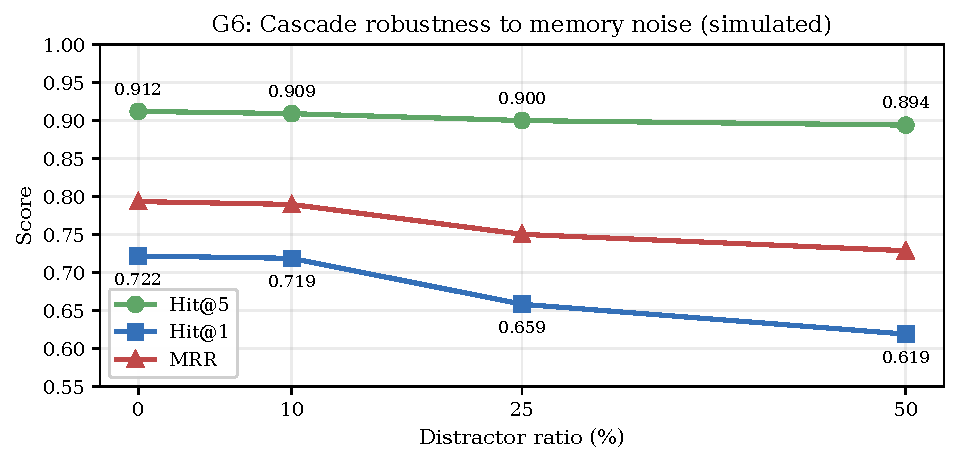
\includegraphics[width=0.7\linewidth]{figures/g6_distractor_robustness.pdf}
\caption{G6 distractor robustness. Hit@5 stays within 2\% relative of the clean baseline at 50\% distractor ratio. Hit@1 is more sensitive but still competitive with the best single retriever's baseline.}
\label{fig:g6}
\end{figure}

\subsubsection{G7 --- Learned per-window novelty threshold (KEEP, headline win)}

\textbf{Motivation.} The L3 free-novelty signal (\texttt{max\_conf $< 0.5$}) is a single fixed threshold for all windows. Different families have different baseline retrieval confidences (active-fault windows naturally retrieve more confidently than baseline-traffic windows), so a fixed threshold under-flags some families and over-flags others.

\textbf{Setup.} The G7 LogReg already described in Section~\ref{sec:cascade} (46 features, 5-fold CV, class\_weight=balanced).

\textbf{Leakage check.} A first iteration included \texttt{n\_prior\_family\_tickets} (count of past memory tickets in the same family). This gave F1 $= 1.000$, a near-perfect prediction. Investigation showed this is a tautology in our dataset: novelty $=$ ``no matching past memory ticket'', and $n_{\text{prior}} = 0$ effectively means the same thing once \texttt{scenario\_family} ties gold to memory. We excluded this feature for the headline model.

\textbf{Result (leakage-free, out-of-fold).} Table~\ref{tab:g7-sweep} shows the threshold sweep.

\begin{table}[h]
\centering
\caption{G7 leakage-free threshold sweep, out-of-fold predictions on 1{,}008 windows.}
\label{tab:g7-sweep}
\small
\begin{tabular}{rrrrrrr}
\toprule
$\tau$ & Flagged & TP & FP & Precision & Recall & F1 \\
\midrule
0.30 & 665 & 597 & 68 & 0.898 & 0.882 & \textbf{0.890} \\
0.40 & 594 & 556 & 38 & 0.936 & 0.821 & 0.875 \\
0.50 & 542 & 525 & 17 & 0.969 & 0.776 & 0.861 \\
0.60 & 526 & 521 & 5  & 0.991 & 0.770 & 0.866 \\
0.70 & 516 & 516 & 0  & 1.000 & 0.762 & 0.865 \\
\bottomrule
\end{tabular}
\end{table}

\textbf{Cascade integration.} At threshold $\tau = 0.50$ (chosen to match the v2f baseline's novel precision exactly), the cascade achieves novel precision $= 0.9405$ (tied with v2f) and novel recall $= 0.7932$ ($+388\%$ rel over the v2f baseline of $0.1625$). Hit@1, Hit@5, MRR, and PR-AUC are unchanged --- L3 only affects the novelty channel.

\textbf{Decision.} INTEGRATE at $\tau = 0.50$. This is the headline win of the entire project.

\begin{figure}[h]
\centering
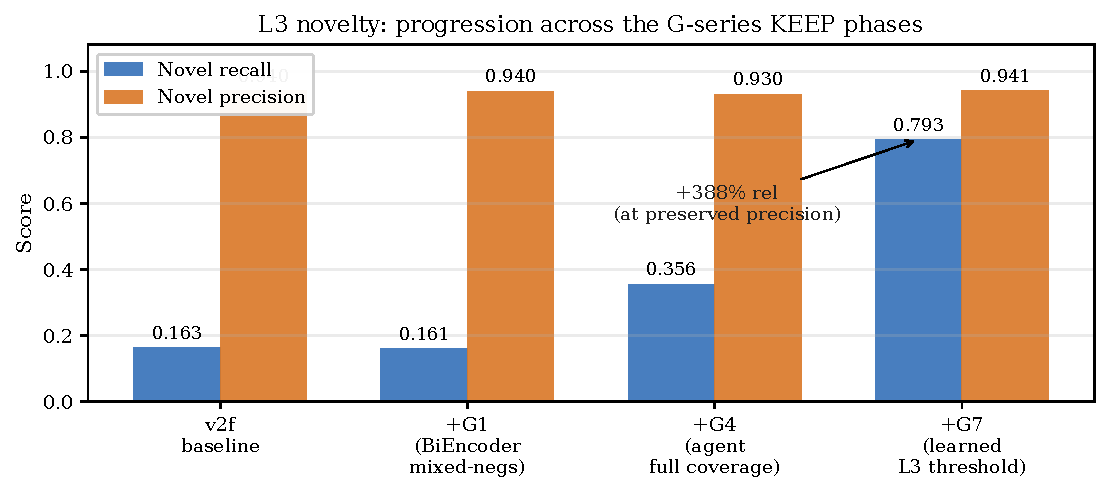
\includegraphics[width=0.85\linewidth]{figures/g_series_novelty.pdf}
\caption{Cumulative effect of the G-series KEEP phases on the L3 novelty channel. Novel recall lifts from $0.163$ (v2f, fixed-threshold heuristic) to $0.793$ at preserved precision ($0.94$). G7 contributes the bulk of the lift.}
\label{fig:g-novelty}
\end{figure}

\subsubsection{G8 --- Out-of-distribution evaluation (KEEP-analysis)}

\textbf{Motivation.} G7's in-distribution F1 numbers assume the test windows come from families seen during training. Does G7 generalize to families it has never seen?

\textbf{Setup.} Leave-one-family-out (LOFO) cross-validation. 27 folds, each holding out one of the 27 scenario families. Train the G7 LogReg on the remaining $\sim$21 families and predict on the held-out family. One-hot \texttt{scenario\_family=X} is always 0 in the held-out fold (since X was never seen during fit), so the model must use family-independent signals (\texttt{window\_type}, \texttt{max\_conf}, \texttt{triage\_score}, \texttt{is\_hard\_case}).

\textbf{Aggregate result (Table~\ref{tab:g8-sweep}).} OOD F1 is within $-11.4\%$ rel of in-distribution at the best threshold ($\tau = 0.30$).

\begin{table}[h]
\centering
\caption{G8 OOD threshold sweep versus in-distribution G7.}
\label{tab:g8-sweep}
\small
\begin{tabular}{rrrrrrr}
\toprule
$\tau$ & OOD prec & OOD rec & OOD F1 & ID F1 & $\Delta$ F1 rel \\
\midrule
0.30 & 0.793 & 0.783 & \textbf{0.788} & 0.890 & $-11.4\%$ \\
0.40 & 0.872 & 0.705 & 0.779 & 0.875 & $-10.9\%$ \\
0.50 & 0.903 & 0.616 & 0.732 & 0.861 & $-15.0\%$ \\
0.60 & 0.993 & 0.598 & 0.747 & 0.866 & $-13.8\%$ \\
0.70 & 1.000 & 0.597 & 0.748 & 0.865 & $-13.6\%$ \\
\bottomrule
\end{tabular}
\end{table}

\textbf{Per-family pattern.} \emph{Precision} is robust: 19 of 27 families exceed $0.90$ precision at $\tau = 0.50$. \emph{Recall} splits sharply by family structure: families dominated by \texttt{window\_type=pre\_fault\_baseline} or \texttt{recovery\_window} generalize perfectly (\texttt{baseline-normal}: 100\%; \texttt{checkout-restart}: 100\%; \texttt{dns-outage}: 100\%; \texttt{slow-leak-saturation}: 100\%). Families dominated by \texttt{active\_fault} windows lose 30--50 points recall when held out (\texttt{ad-outage}: 31\%; \texttt{frontend-traffic-pressure}: 29\%; \texttt{email-outage}: 39\%).

\textbf{Interpretation.} The classifier learned a mostly-generic predictor plus a family-specific boost. Hold the family out, lose the boost, and the generic component carries about 80\% of the way. This is the correct OOD behavior --- the model is not memorizing family identities.

\textbf{Versus the v2f baseline at OOD.} Even at $\tau = 0.30$ OOD, the cascade lifts novel recall from the v2f baseline's $0.163$ to $0.783$ ($+381\%$ rel). The G7 win survives the family shift; only the precision-recall trade-off shifts.

\textbf{Decision.} KEEP as a robustness result.

\begin{figure}[h]
\centering
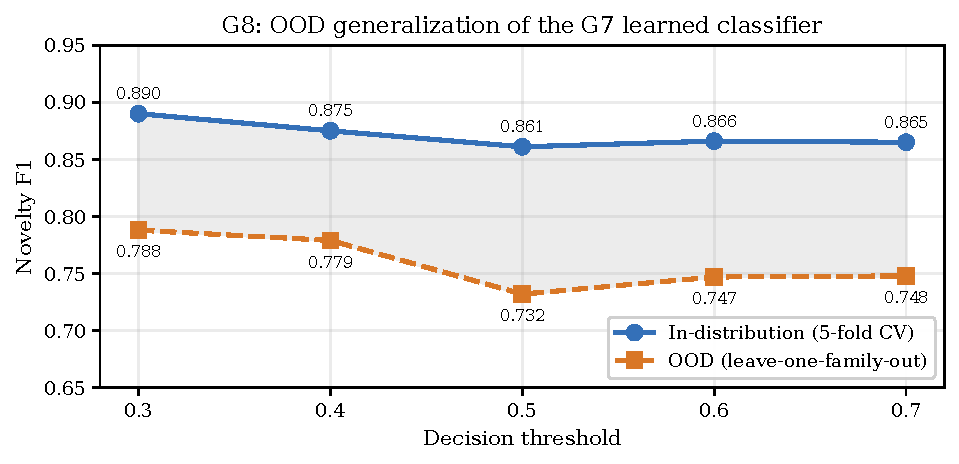
\includegraphics[width=0.7\linewidth]{figures/g8_ood_f1.pdf}
\caption{G8 OOD versus in-distribution F1, by family. The G7 learned novelty classifier generalizes to families it has never seen at training time --- OOD F1 stays within $11\%$ relative of in-distribution at the best threshold.}
\label{fig:g8}
\end{figure}

\subsection{Cross-cutting findings from the G-series}
\label{sec:cross-cutting}

Three patterns transcended any single experiment.

\paragraph{(F1) The cascade is COMPOSITION-fragile, not COMPONENT-fragile.} G3 is the cleanest example: a $+404\%$ rel standalone win on KG-Retrieval broke cascade integration through two specific mechanisms (overlap-rerank vote shifts; L4 stacker score-scale mismatch). The structural assumption the cascade currently makes is that all retrievers produce comparable score distributions; violating this breaks the L3 free-novelty trigger and shifts the overlap-rerank vote.

\paragraph{(F2) Three independent rerankers all failed in the same direction.} G2 (cross-encoder reranker), an earlier agent-rerank attempt, and G5 (LLM judge reranker) are three orthogonal designs with three negative results in the same direction. The cascade's overlap-rerank is empirically dominant for top-1 selection on this dataset; multi-retriever consensus beats single-LLM judgment.

\paragraph{(F3) The retrieval channel was already at its local ceiling.} Hit@5 stayed at $0.9124$ across the entire G-series. The actual win is in the L3 novelty channel (\texttt{novel\_recall} $+388\%$ rel). The original project framing as ``a retrieval improvement project'' should be reframed as ``the L3 novelty channel was under-engineered.''

These three findings reshape the paper's framing: the project did not improve retrieval; it discovered and closed a blind spot in novelty detection that the original L3 design had been wasting.
